\chapter{Интеллектуальные системы регистрации и анализа проблемных ситуаций, возникающих в ИТ-инфраструктуре предприятия} \label{chapt1}

\section{Обзор исследований в области интеллектуальных систем регистрации и анализа проблемных ситуаций} 
В данной главе рассматриваются постановка задачи и обзор исследований в области интеллектуальных систем регистрации и анализа проблемных ситуаций. \par

\textbf{Постановка задачи.} Большинство проблем, которые решает удаленная служба поддержки информационной инфраструктуры предприятия, носит достаточно тривиальный характер (по данным компании \icl): установить приложение; переустановить приложение; решить проблему с доступом к тому или иному ресурсу.
Названные проблемы решают специалисты технической поддержки, которая обычно делится на несколько линий по уровню умения специалистов (см. таблицу \ref{TSSDescription}). Каждая линия поддержки представлена своим классом специалистов. В среднем команда, обслуживающая одного заказчика, насчитывает около 60 человек. Процентное соотношение специалистов разных линий поддержки отображено на рисунке \ref{img:ITSMTeamComposition}.

\begin{longtable}{|p{4cm}|p{12cm}|}
 \caption[Описание работы специалистов различных уровней поддержки]{Описание работы специалистов различных уровней поддержки}\label{TSSDescription} \\ 
 \hline\multicolumn{1}{|c|}{\textbf{Уровень}} & \multicolumn{1}{c|}{\textbf{Описание}} \\ \hline 
\endfirsthead
\multicolumn{2}{c}%
{{\bfseries \tablename\ \thetable{} -- продолжение}} \\
\hline\multicolumn{1}{|c|}{\textbf{Уровень}} & \multicolumn{1}{c|}{\textbf{Описание}} \\ \hline 
\endhead
\endfoot

\hline \hline
\endlastfoot
  \hline
Первая линия	& Решение уже известных, задокументированных проблем, работа напрямую с пользователем \\
  \hline
Вторая линия  & Решение ранее неизвестных проблем \\
  \hline
Третья линия & Решение сложных и нетривиальных проблем \\
  \hline
Четвертая линия  & Решение архитектурных проблем инфраструктуры \\
 
\end{longtable}



\begin{figure} [h] 
  \center
  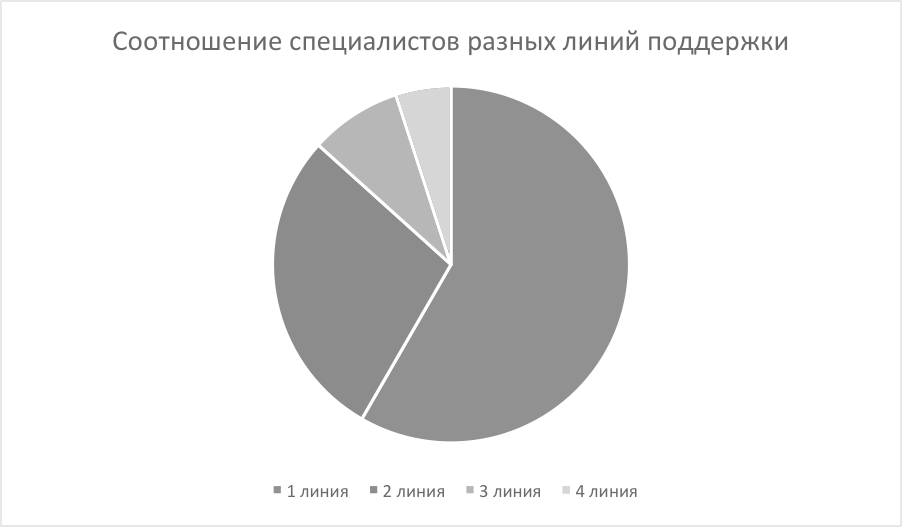
\includegraphics [scale=0.8] {ITSMTeamComposition}
  \caption{Диаграмма состава команд} 
  \label{img:ITSMTeamComposition}  
\end{figure}

Работа специалистов первой линии поддержки состоит из множества рутинных и простых задач. На рисунке \ref{img:EngineerTasks} показано соотношение разных типов проблем, встречающихся во время работы службы поддержки, в таблице \ref{IncidentDescription} приведена расшифровка типов. Данные подготовлены на основе анализа работы команд \icl.


\begin{figure} [h] 
  \center
  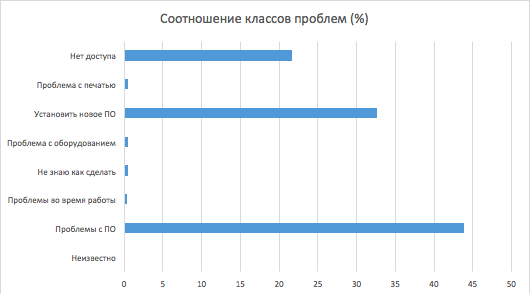
\includegraphics [scale=1.0] {EngineerTasks}
  \caption{Диаграмма соотношений типов проблем} 
  \label{img:EngineerTasks}  
\end{figure}



\begin{longtable}{|p{6cm}|p{10cm}|}
 \caption[Категории инцидентов в области удаленной поддержки инфраструктуры]{Категории инцидентов в области удаленной поддержки инфраструктуры}\label{IncidentDescription} \\ 
 \hline\multicolumn{1}{|c|}{\textbf{Категория}} & \multicolumn{1}{c|}{\textbf{Описание}} \\ \hline 
\endfirsthead
\multicolumn{2}{c}%
{{\bfseries \tablename\ \thetable{} -- продолжение}} \\
\hline\multicolumn{1}{|c|}{\textbf{Категория}} & \multicolumn{1}{c|}{\textbf{Описание}} \\ \hline 
\endhead
\endfoot

\hline \hline
\endlastfoot
  \hline
Проблема с ПО	& Проблема при запуске ПО на компьютере. Решается переустановкой \\
  \hline
Проблемы во время работы  & Проблема с функционированием программного обеспечения\\
    \hline
Как сделать & Запрос на инструкцию по работе с тем или иным компонентом рабочей станции \\
      \hline
Проблема с оборудованием  & Неполадки на уровне оборудования \\
  \hline
Установить новое ПО       & Требование установки нового программного обеспечения \\
  \hline
Проблема с печатью        & Установка принтера в систему \\
    \hline
Нет доступа               & Нет доступа к общим ресурсам \\
 
\end{longtable}

Как показывают исследования, решение части задач может быть автоматизировано. Если это будет сделано,  специалисты получат дополнительное время для решения более сложных задач. \par

\textbf{Применение моделей теории массового обслуживания}\par
Рассмотрим модель данной системы в разрезе теории массового обслуживания (ТМО). Она может быть выражена в виде входящего потока заявок (инцидентов), очереди и нескольких агентов (специалистов, автоматизированных систем). 
Важно отметить, что на время обработки заявки агент блокируется и не может принимать новые заявки. На рисунке \ref{img:mass_service} представлена модель системы массового обслуживания в ИТ, в которой использованы следующие обозначения рассматриваемых величин $\lambda$ --- интенсивность входящего потока;
$\alpha$ --- доля заявок, для которых время в очереди превышает $max(T_q)$;       
$\mu$ --- величина, обратная среднему времени нахождения заявки у агента;
n --- число агентов;
$T_q$ --- время нахождение заявки в очереди в часах;
SLA --- уровень обслуживания (1-$\alpha$), доля заявок, для которых время в очереди не превышает $max(T_q)$. $T_p$ --- время удовлетворения заявки;
 $\alpha_n$ --- количество заявок;
 $T_{qp}=T_q+T_p$ --- время прохождения заявки через систему;
 $S(\mu)= \frac{R_p}{\mu} $ --- средняя стоимость выполнения одной заявки;
 $R_p$ --- средняя стоимость часа работы специалиста (выводится далее).

  
\begin{figure} [h] 
  \center
  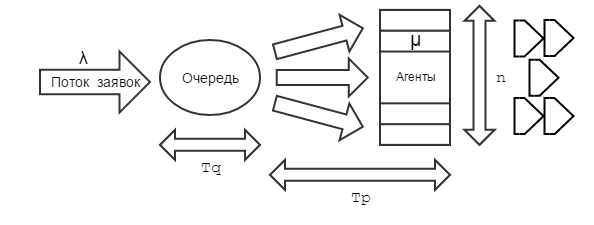
\includegraphics [scale=0.8] {mass_service}
  \caption{Модель системы массового обслуживания в ИТ.} 
  \label{img:mass_service}  
\end{figure}

Существует несколько подходов решения задач ТМО: 
\begin{itemize}
	\item Аналитическое решение для простейших систем, которое позволяет выразить $T_q (t)$ через $\lambda$, $\mu$ и $n$;
	\item Решение с помощью имитационного подхода, где строится гистограмма $T_q (t)$, по которой оценивается достаточность $n$ для обеспечения SLA;
	\item Решение с помощью эконометрического подхода, которое подходит для систем с достаточно большим $n$. В таких системах возможно оценить $T_q (t)$ по имеющейся статистике.
\end{itemize} \par
В \cite{TMO} на основе комбинации формулы Эрланга, модели Энгсета и модели Полячека~--~Хинчина 
построена формула для решения задач ТМО на основе аналитического подхода путем нахождения распределения вероятностей для $T_qp$. Основной же задачей этой работы является прогнозирование необходимых ресурсов для максимизации $SLA$~ ($SLA=1-\alpha$). 
В данной диссертации ставится задача минимизации $T_{qp}$, $S(\mu)$ и динамического выделения ресурсов. На основе  статистики, собранной в компании \icl,~ был подсчитан следующий коэффициент $T_{qp}=47,9$ при $n=6$; $SLA=0,82$; $\alpha=0,18$;  $\alpha_n=2920$. 
Для анализа потока заявок в данном случае лучше использовать имитационный подход, так как $n$ слишком мало. На рисунке \ref{img:LAMBDAAV} представлен средний поток заявок по часам, посчитанный на основе собранной статистики. На нем наглядно видно, как изменяется поток с течением дня. Пик обращений от пользователя приходится на промежуток между 13:00 и 16:00.

\begin{figure} [h] 
  \center
  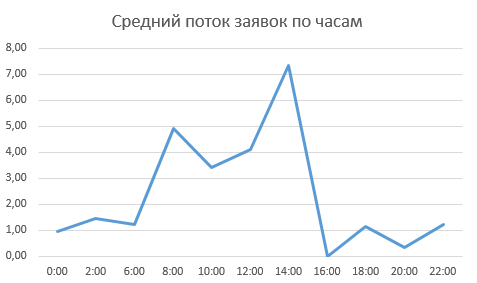
\includegraphics [scale=1.0] {LAMBDAAV}
  \caption{Средний поток заявок по часам.} 
  \label{img:LAMBDAAV}  
\end{figure}


\textbf{Оценка стоимости работы специалиста}\par По данным аналитики портала SuperJob \cite{SuperJob}, в Казани средняя зарплата системного администратора с опытом работы в 2014 году составляла 30 – 35 тыс. руб. (с учетом 21 рабочего дня в месяце~--- 179--208 руб. в час). В соответствии с действующим российским законодательством \cite{FiscalCodecs} расходы компании на одного работника определяются по формуле
\[
L = R + R*(F_1 +F_2+F_3),
\]
где $R$~--- выплата человеку в час, $F1$~--- НДФЛ 13\%, $F2$~--- совокупность отчислений в ФБ (6\%), ПФР (14\%), ТФОМС (2\%), ФФОМС (1,1\%), ФСС (2,9\%), $F3$~--- налог на прибыль (20\%). Таким образом, расходы компании на сотрудника варьируются от 285 до 314 руб. в час, а за 8-ми часовой рабочий день – от 2280 до 2512 руб. Далее, аренда выделенного сервера (такого, например, как Xeon X3, 1.7 GHz, 8GB RAM, 256GB SSD) стоит 8 900 руб./мес. (см. \cite{TimeWeb}) (53 рубля за 1 час, с учетом 8-ми часового рабочего дня $R_p=53$). Но сервер может работать 24 часа в сутки за исключением простоев на обслуживание, которые обычно составляют не более 5\% времени. \par

 Итого: сервер работает 478,8 часов в месяц. С этой точки зрения эксплуатация сервера будет стоить 18,5 руб. в час ($R_p=18,5$). Один сервер в своем быстродействии может заменить несколько специалистов при решении соответствующих задач. Чтобы решение было экономически эффективным, необходимо, чтобы оно сокращало расходы как минимум на 30\% (по данным \icl). \par 
 
 Подсчет на основе стоимости часа и пропорции показывает, что работа специалиста~--- это 6\% работы виртуального агента, т.е. сервера (без учета работы сервера параллельно над несколькими задачами). Таким образом, уровень разрешения инцидентов системой в 30\% выполнит требования по прибыли примерно на 111\%.

\textbf{Предпосылки развития изучаемой предметной области}\par 
Основной тенденцией в развитии области удаленной поддержки ИТ-инфраструктуры являются попытки удешевить и улучшить стоимость предоставления услуг \cite{OutsourceEff}. \par
Компании, работающие на этом рынке, вкладывают большие средства в автоматизацию. Кроме того, современное развитие науки и техники, точнее, вычислительных мощностей \cite{SuperComputer} позволяет провести автоматизацию даже самых наукоемких процессов. Дальнейшей перспективой развития области удаленной поддержки ИТ-инфраструктуры является замена человеческих специалистов автоматизированными системами. Разработки в этом направлении ведут многие компании, например, компания HP, которая имеет свою систему регистрации различных инцидентов \cite{HPOpenView} и сейчас ведет работу над ее автоматизацией. В качестве некоторого сравнения можно провести параллель происходящего процесса с промышленной революцией XVIII–XIX веков (см., например, \cite{IndustrialRev}). \par
\textbf{Обзор исследований в изучаемой предметной области}\par Область исследования, с которой связана диссертация, является комплексной и включает в себя различные направления работ, в частности, создания различных интеллектуальных систем. Сфера применения интеллектуальных систем обширна, например, в Институте Чиная (Индия) Е. Джубилсоном и П. Дханавантини ведутся исследования интеллектуальных систем обработки запросов пользователей в области телекоммуникаций \cite{CHIN-1}, а в университете Ганновера (Германия) Р. Брунс и Дж. Данкель разрабатывают интеллектуальные системы для обработки запросов в службу спасения с целью уменьшения времени реакции на происшествие \cite{Dunkel}. В Санкт-Петербургском государственном университете под руководством В.И. Золотарева проводится оценка эффективности службы информационной поддержки в Вычислительном центре СПбГУ \cite{SPB}. В Сингапуре С. Фу и П. Леонг проведен анализ эффективности ИТ-службы поддержки крупной компании и показана возможность автоматизации ряда процессов \cite{SING}.\par
Исследования в области интеллектуальных систем повышения эффективности ИТ-службы предприятия ведутся также лидерами отрасли: компаниями HP \cite{HPOpenView} и IBM \cite{WATSON-PO}. Например, известна многоцелевая интеллектуальная система IBM Watson, разработкой и исследованием которой занимается группа под руководством профессора А. Гоэля (США--Китай).  \par   

Еще одно из направлений исследований в области обработки естественного языка составляет подход GATE \cite{GATE-1}, который активно развивается в университете Шеффилда (Великобритания) под руководством Г. Каллаган, Л. Моффат и С. Сзаз. Другое направление~--- это семантический поиск, исследования в этой области также активно ведутся в университете Шеффилда, в частности, выработан подход "Mimir"\,, который реализует возможности поиска по принципу «поиск и открытие» \cite{MIMIR}. Для организации поиска решений в соответствии с запросами пользователей в таких системах используются онтологии, например, широко применяется подход, предложенный С. Дей и А. Джеймс из Калифорнийского университета (США), основанный на применении деревьев тегов в онтологии \cite{ONTCON}. \par
Для придания интеллектуальной системе гибкости необходимо дать ей возможность проводить логические рассуждения. Одной из ведущих организаций в этом направлении исследований является консорциум OpenCog \cite{OpenCog} (США). Этими работами руководит Бен Герцель (председатель Artificial General Intelligence Society и OpenCog Foundation)~--- один из мировых лидеров в области искусственного интеллекта. Исследования в области машинной логики также ведутся в рамках проекта NARS \cite{NARS} под руководством профессора университета Темпла (США) Пея Вонга. \par 

Интерес к области интеллектуальных систем обработки информации можно, в частности, оценить как количество публикаций за последние годы, процитированных в базе данных Scopus,~--- с 2004 года в среднем оно составило около 1010 в год. \par
\textbf{Стандарты, используемые в области ИТ-аутсорсинга: ITIL и ITSM} \par
В области ИТ-аутсорсинга есть несколько готовых стандартов ведения работ, одним из которых является библиотека ITIL. Этот стандарт описывает лучшие практики организации работ в области ИТ-аутсорсинга. Используемый в библиотеке подход соответствует стандартам ISO 9000 (ГОСТ Р ИСО 9000) \cite{ITIL1, ITIL2, ITIL3}.
Наличие стандартов диктует унифицированность как постановки проблем, так и алгоритмов решения, а также способствует возможности частичной или в некоторых случаях полной автоматизации решения проблем. \par
\clearpage


\section{Сравнительный анализ систем регистрации и устранения проблемных ситуаций} \label{sect3_2}
\textbf{HP OpenView} \cite{HPOpenView, HP1, HP2, HP3} является комплексным программным решением по мониторингу ИТ-инфраструктуры предприятия и имеет множество модулей. На рисунке \ref{img:hpopenview} представлен вид системы, которая обладает широким спектром возможностей: мониторинг \cite{HP4, HP5}; регистрация инцидентов; управление системами. Система не поддерживает: понимание и формализацию запросов; автоматическое устранение проблемы на основе формализации запроса.

\begin{figure} [h] 
  \center
  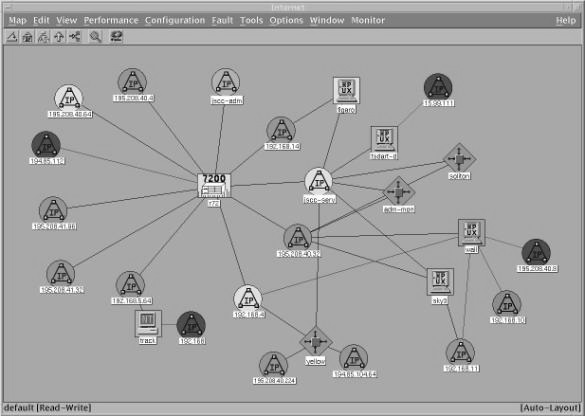
\includegraphics [scale=1.0] {hpopenview}
  \caption{HP OpenView (материал из Wikipedia)} 
  \label{img:hpopenview}  
\end{figure}

Система \textbf{ServiceNOW}\footnote{Система ServiceNOW \url{http://www.servicenow.com/}}~--- средство автоматизации сервиса. На рисунке \ref{img:svnow} представлен вид этой системы, которая предоставляет следующие возможности: регистрация инцидентов и создание цепи их обработки. Система не поддерживает: понимание и формализацию запросов; автоматическое исправление проблемы на основе формализации запроса. Система широко используется в ИТ-инфраструктуре CERN \cite{SN1, SN2} для регистрации инцидентов и их решения.

\begin{figure} [h] 
  \center
  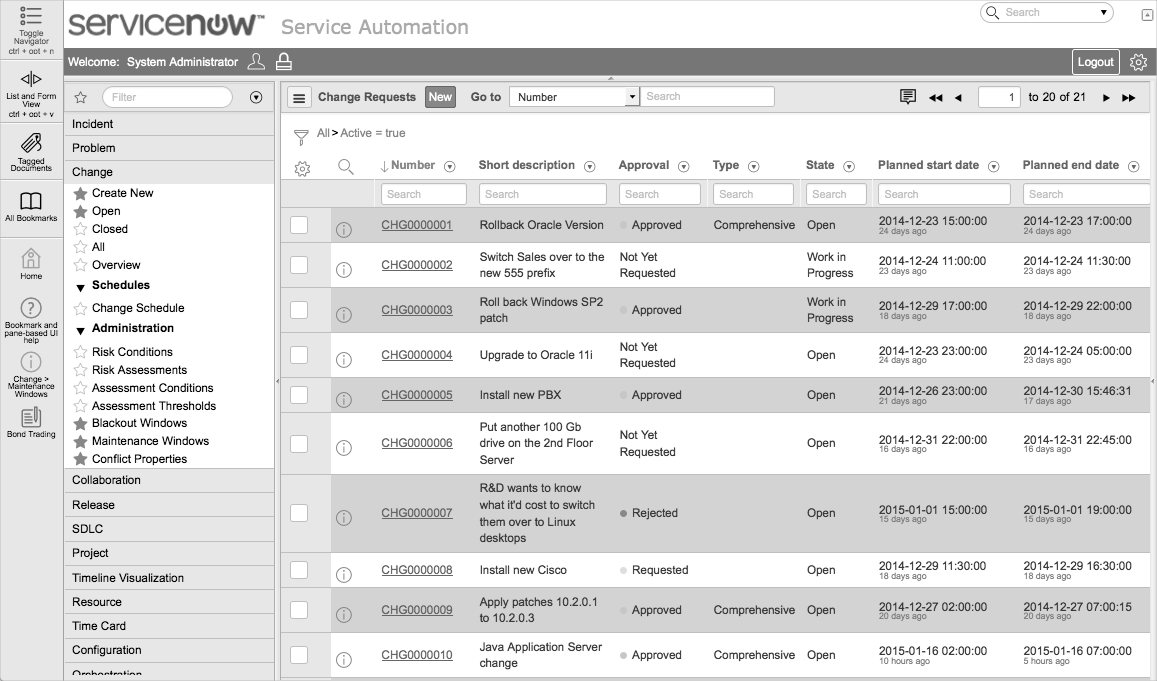
\includegraphics [scale=0.3] {svnow}
  \caption{Service NOW (материал из http://wiki.servicenow.com/)} 
  \label{img:svnow}  
\end{figure}

\textbf{IBMWatson}~--- это вопросно-ответная система, которая поддерживает понимание и формализацию запросов и поиск решений. Система не поддерживает автоматическое разрешение проблемы на основе формализации запроса. Система широко используется в медицине для постановки диагнозов болезней \cite{IBM1, IBM2, IBM3, IBM4} и реализует базовые принципы искусственного интеллекта \cite{IBM5, IBM6}. Ее разработка велась под суперкомпьютер IBM Deep Blue \cite{IBM7} группой под руководством профессора А. Гоэля. На рисунке \ref{img:Watson-Analytics} представлен общий вид этой системы. \par


\begin{figure} [h] 
  \center
  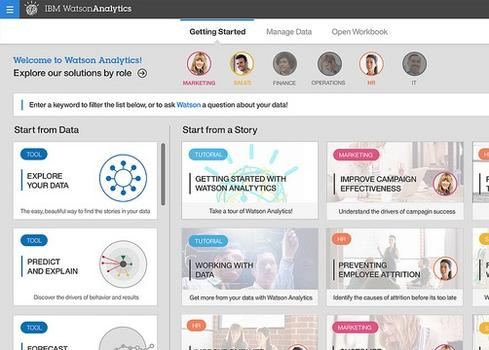
\includegraphics [scale=1.0] {Watson-Analytics}
  \caption{Пример работы системы Watson (материал из http://www.informationweek.com/)} %http://www.informationweek.com/cloud/software-as-a-service/ibm-watson-data-analysis-service-revealed/d/d-id/1315769
  \label{img:Watson-Analytics}  
\end{figure}

Кроме того, известны следующие дополнительные способы и системы автоматизации разрешения проблемы пользователя:
\begin{itemize}
	\item Обработка инцидентов посредством регулярных выражений. В таком решении нет гибкости, так как обработка идет путем поиска ключевых слов вне контекста. Метод регулярных выражений частично используется для обработки естественного языка, поиска  \cite{REG1}, диагностики активных систем \cite{REG2}, анализа поведения функций \cite{REG4}, обработки данных в системе eDiscovery \cite{REG5}, в разработке способов программирования \cite{REG3};
	\item Обработка инцидентов при помощи скриптов~--- автоматизируются лишь рутинные операции.
\end{itemize} \par
На данный момент времени ни одна из описанных систем в полной мере автоматически не разрешает запросы пользователей: не фиксирует их, не проводит анализ, не ищет решение, не применяет решение и не дает обратной связи пользователю. Каждая система в той или иной мере реализует те или иные функции, но системы, которая реализует их все, пока не существует. \par

Для того чтобы создать модель системы, необходимо определить требования к ней или критерии, соответствие которым будет служить одним из доказательств состоятельности системы наряду с экспериментальными результатами. \par

Перечисленные ниже требования сформированы, исходя из возможностей специалистов службы поддержки, а также анализа проблем, которыми они занимаются. Большинство инцидентов~--- тривиальные и типичные, но все они разные. Для человека проблемы ”Please install Firefox” и ”Please install Chrome” идентичны, но с точки зрения формализации это не так~--- общее в них можно найти, взглянув на обобщение различающейся части: Firefox и Chrome являются пакетами программного обеспечения. \par 
Чтобы понять, каким требованиям должны соответствовать интеллектуальная система регистрации и анализа проблемных ситуаций в ИТ-области, нужно понять, что делает специалист службы поддержки. Такой специалист регистрирует проблему, анализирует, ищет решение, проводя логические рассуждения и фиксируя в памяти удачное решение, и решает проблему. Итак, чтобы обеспечить полностью автоматическое разрешение инцидентов, интеллектуальная система регистрации и анализа проблемных ситуаций в ИТ-области должна соответствовать следующим критериям: осуществлять мониторинг ИТ-инфраструктуры пользователя; регистрировать инциденты; создавать цепи обработки (Workflow) инцидента; понимать и формализовать запросы пользователя на естественном языке; искать решение и применять найденное решение; обучаться алгоритму разрешения инцидента; уметь проводить логические рассуждения (обобщение, специализация, синонимичный поиск). \par
Из этого списка требований к системе важно выделить формализацию запросов на естественном языке. Ниже приведены результаты анализа разработок в области формализации запросов на естественном языке. 


\section{Сравнительный анализ методов и комплексов обработки текстов на естественном языке}


\subsection{Обработка эталонных текстов} \label{sect2_1}
В данном разделе проведен обзор обработчиков естественного языка. За основу были взяты инциденты, выгруженные из систем поддержки ИТ-инфраструктуры \icl. В силу специфики предметной области (информационные технологии) основным языком был выбран английский язык. Был сформирован список из типичных эталонных фраз, на которых тестировались обработчики естественного языка. Фразы были выявлены путем анализа существующих отчетов об инцидентах. Примерами инцидентов являются следующие запросы.\par
\textbf{Инцидент 1}.
\textit{
User had received wrong application. User has ordered Wordfinder Business Economical for her service tag 7Q4TC3J, there is completed order in LOT with number ITCOORD-18125. However she received wrong version, she received Wordfinder Tehcnical instead of Business Economical. Please assist (Пользователю было установлено неверное приложение. Пользователь заказал приложение "Wordfinder Business Economical"\  для ее запроса номер 7Q4TC3J. По нашим данным запрос выполнен, номер результата ITCOORD-18125. Однако, он получил неверную версию~--- он получил приложение "Wordfinder Tehcnical"\  вместо "Wordfinder Business Economical". Пожалуйста, помогите).\footnote{Здесь и далее в переводе оригинальные синтаксические, грамматические и стилистические ошибки сохранены, дабы продемонстрировать сложность формализации запросов на естественном языке.}
}\par
\textbf{Инцидент 2}.
\textit{
Laptop~--- user has almost full C:\ but when he looks in the properties of the files and folders on C:\ they are only 40~Gb and he has a 55~Gb drive (Ноутбук~--- диск C:\ пользователя переполнен, но он посмотрел свойства C:\ и увидел, что имеется только 40~Gb, хотя пользотель установил накопитель на 55~Gb).
}\par
\textbf{Инцидент 3}.
\textit{
User cannot find Produkt Manageron start menu. Please reinstall (Пользователь не может найти Produkt Manageron в меню "Пуск". Пожалуйста, переустановите). 
}\par
\textbf{Инцидент 4}.
\textit{
User needs to have pdf 995 re-installed please (Пользователю нужно переустановить "pdf 995").
}\par

При анализе этих запросов были использованы следующие обработчики естественного языка: Open NLP \cite{OpenNLP}, Relex\cite{OpenCogRelex}, StanfordParser \cite{StanfordParser}. Результат их работы оценивался при помощи метрик, представленных в таблице \ref{Metrics}, а полученные результаты приведены на рисунке \ref{img:ParserComp}. 

\begin{longtable}{|p{2cm}|p{6cm}|p{8cm}|}
 \caption[Таблица метрик]{Таблица метрик}\label{Metrics} \\ 
 \hline
 
 \multicolumn{1}{|c|}{\textbf{Метрика}} & \multicolumn{1}{c|}{\textbf{Описание}} & \multicolumn{1}{c|}{\textbf{Формула}} \\ \hline 
\endfirsthead
\multicolumn{2}{c}%
{{\bfseries \tablename\ \thetable{} -- продолжение}} \\
\hline\multicolumn{1}{|c|}{\textbf{Метрика}} & \multicolumn{1}{c|}{\textbf{Описание}} & \multicolumn{1}{c|}{\textbf{Формула}}  \\ \hline 
\endhead
\endfoot

\hline \hline
\endlastfoot
  \hline

Precision	& Точность & 
$$ 
P=\frac{tp}{tp+fp},
$$ где $P$~--- precision, $tp$~---  успешно обработанные слова, $fp$~--- ложно успешные \\
 \hline
Recall	& Чувствительность & 
$$ 
R=\frac{tp}{tp+fn},
$$ где $R$~--- recall, $tp$~--- успешно обработанные слова, $fn$~--- ложно неуспешные \\
 \hline
$F$	& $F$~--- measure (результативность) & 
$$ 
F=\frac{P*R}{P+R},
$$ где $P$~--- precision, $R$~--- recall.   \\
 
\end{longtable}

\begin{figure} [h] 
  \center
  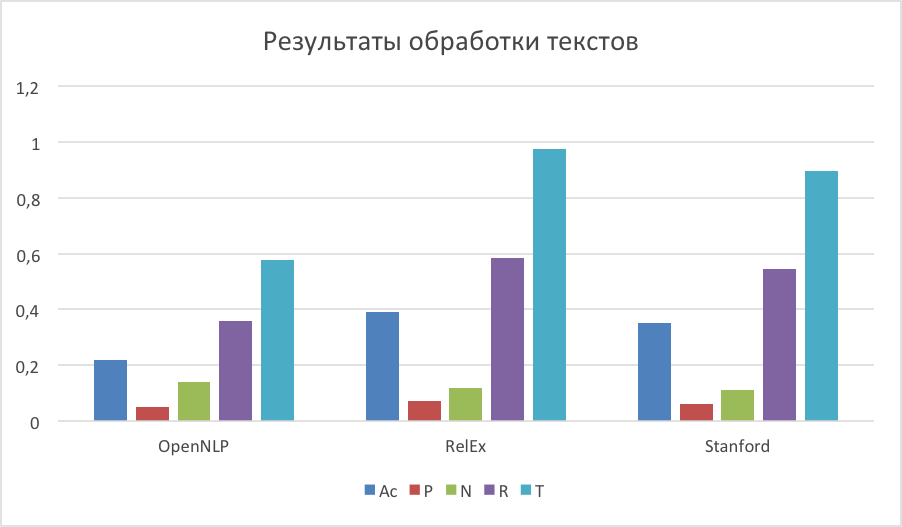
\includegraphics [scale=0.8] {ParserCompare}
  \caption{Результаты обработки текстов} 
  \label{img:ParserComp}  
\end{figure}

Из диаграммы \ref{img:ParserComp} видно, что наилучшие результаты показывает обработчик Relex\cite{OpenCogRelex}. После анализа необработанных инцидентов у всех обработчиков были выявлены проблемы двух типов:
\begin{enumerate}
	\item невозможность корректировки простых грамматических ошибок, связанных с пропущенными пробелами или неверным форматированием (ошибки первого типа);
	\item полисемия, например, слово please интерпретировалось как глагол, хотя является по смыслу «вводным словом» (ошибки второго типа).
\end{enumerate}	\par

Несмотря на хорошие результаты~--- 63\% успешно разобранных предложений, ошибки первого и второго типов серьезно ухудшают результат. Эффективность разбора предложений в 63\% случаев недостаточна для успешной работы системы. Чтобы улучшить показатель, был разработан комплекс мер для устранения ошибок первого и второго типов.
	
 
\subsection{Исправление ошибок первого и второго типов} \label{sect2_2}
Чтобы разрешить проблемы, связанные с ошибками первого и второго типов, была проведена предварительная обработка текста, состоящая из 2-х фаз: комплексная корректировка~--- для ошибок первого типа; обработка при помощи внутренней базы знаний~--- для ошибок второго типа. 
Чтобы избавиться от орфографических, грамматических и синтаксических ошибок, был сконструирован составной корректировщик, который имеет модульную структуру и осуществляет корректировку последовательно в рамках выбранной области знаний (например, одного проекта). В результате были сконструированы модули корректировки: Google API~--- модуль подключения к открытым системам Google для использования их алгоритмов корректировки; After the Deadline~--- модуль, использующий открытый программный продукт After the Deadline для исправления текстов. 

Таким способом удалось исправить большинство ошибок, связанных с синтаксисом, грамматикой и орфографией в рамках выбранной области (корректировка ошибок в ограниченной области гораздо проще, чем универсальная корректировка). Также удалось исправить ошибки неверного написания: наличия лишних пробелов, пропуска запятых и точек в виду лаконичности входной информации. Необходимо отметить, что входная информация представляет собой простые предложения в рамках терминологии одной области знаний (ИТ, специфические термины, которые используются только на этом проекте), что значительно упрощает корректировку ошибок. По-прежнему осталась проблема обработки неверной интерпретации слов в тексте (полисемии). \par

Для корректировки ошибок второго типа был сконструирован модуль для обработчика естественного языка Relex, который разбивал стандартный процесс обработки на «предобработку» и «обработку». Стадия «обработки» включает в себя такой же алгоритм работы, как был до этого в модуле Relex, а стадия «предобработки» проверяет входные данные (слово или предложение) на предмет его вхождения во внутреннюю базу знаний, и если таковое имеется, то приложение передает соответствующие корректировки обратно в модуль. Например, Relex во фразе "please install firefox"\ считает, что "please"\ --- это глагол, поэтому в базе знаний нашей системы отмечено, что "please"\ --- это форма вежливости (проблема полисемии), тем самым Relex больше не интерпретирует "please"\ как глагол в выбранной области знаний (то есть для всех случаев).


\subsection{Сравнение средств обработки русского и английского языков} \label{sect2_3}
Средства обработки естественного языка принято относить к большому классу средств NLP~--- Natural Language Processing \cite{NLP}. Для английского языка существует множество открытых средств обработки этого языка, для русского языка найти их гораздо сложнее. Рассмотрим архитектуру средств обработки естественного языка на примере популярного комплекса обработки~--- OpenCog Relex \cite{OpenCogRelex}. \par
OpenCog Relex использует результаты работы открытого компонента для лексического анализа под названием Link Grammar \cite{linkgrammar}. Он поддерживает множество языков: английский, русский, турецкий, немецкий \etc\  В качестве формата вывода Relex использует синтаксис Link Grammar и преобразует его в формат связей, как показано в примере 1. Разбор примера приводится далее. 

\textbf{Пример 1}. User is unable to start KDP web, please reinstall Java.\\
\textbf{Результат} 
\begin{lstlisting}
_obj(start, KBP)
pos(start, verb)
inflection-TAG(start, .v)
tense(start, present)
pos([web], WORD)
noun_number(KBP, singular)
definite-FLAG(KBP, T)
pos(KBP, noun)
_advmod(reinstall, please)
pos(reinstall, verb)
inflection-TAG(reinstall, .v)
tense(reinstall, present)
pos(please, adv)
inflection-TAG(please, .e)
noun_number(Java, singular)
definite-FLAG(Java, T)
pos(Java, noun)
pos(., punctuation)
_obj(,, Java)
pos(,, verb)
tense(,, infinitive)
HYP(,, T)
_to-do(unable, ,)
pos(unable, adj)
inflection-TAG(unable, .a)
tense(unable, present)
pos(to, prep)
inflection-TAG(to, .r)
pos(be, verb)
inflection-TAG(be, .v)
_predadj(User, unable)
noun_number(User, singular)
definite-FLAG(User, T)
pos(User, noun)
\end{lstlisting}




Далее проведем разбор слова start. В результате мы получим несколько отношений:
\begin{itemize}
	\item pos(start, verb)~--- start глагол;
	\item tense(start, present)~--- время настоящее;
	\item inflection-TAG(start, .v)~--- метод обозначения на схеме (индекс).
\end{itemize} \par
Остальные обработчики пока не поддерживают русский язык. Существуют открытые проекты, но они еще недостаточно развиты. Таковым является, например, русский словарь для LinkGrammar \footnote{\url{http://www.abisource.com/projects/link-grammar/russian/}}, но он не доступен для скачивания. 




\section{Выводы по главе 1}
В данной главе рассмотрены существующие на данный момент интеллектуальные системы регистрации и анализа проблемных ситуаций, возникающих в процессе функционирования ИТ-инфраструктуры предприятия.
 В таблице \ref{Comparsion} приведены сводные данные по системам. По ним можно сказать, что ни одна из рассмотренных систем полностью не реализует все необходимые функции для интеллектуальной системы разрешения проблемных ситуаций в ИТ-инфраструктуре предприятия. В главе 1 также выработаны критерии сравнения обработчиков естественного языка и выполнен анализ средств обработки естественного языка. По полученным показателям эффективности было решено использовать OpenCog Relex.

\begin{longtable}{|p{6cm}|p{0.5cm}|p{0.5cm}|p{0.5cm}|}
 \caption[Сравнительный анализ функциональности существующих решений]{Сравнительный анализ функциональности существующих решений}\label{Comparsion} \\ 
 \hline
 
 \multicolumn{1}{|c|}{\textbf{Сравнительный пункт}} & \multicolumn{1}{c|}{\textbf{HP Open View}} & \multicolumn{1}{c|}{\textbf{ServiceNOW}} & \multicolumn{1}{c|}{\textbf{IBM Watson}} \\ \hline 
\endfirsthead
\multicolumn{2}{c}%
{{\bfseries \tablename\ \thetable{} -- продолжение}} \\
\hline \multicolumn{1}{|c|}{\textbf{Сравнительный пункт}} & \multicolumn{1}{c|}{\textbf{HP Open View}} & \multicolumn{1}{c|}{\textbf{ServiceNOW}} & \multicolumn{1}{c|}{\textbf{IBM Watson}}  \\ \hline 
\endhead

\hline \multicolumn{4}{|r|}{{Продолжение следует}} \\ \hline
\endfoot

\hline \hline
\endlastfoot
\hline
   Мониторинг & Да & Да & Да \\
   \hline
   Регистрация инцидентов & Да & Да & Да\\
   \hline
   Управление системами & Да & Нет & Нет \\
   \hline 
   Создание цепи обработки (Workflow) инцидента & Да & Да & Нет \\
   \hline 
   Понимания и формализация запросов на естественном языке & Нет & Нет & Да \\
   \hline 
   Поиск решений & Нет & Нет & Да \\
   \hline 
   Применение решений & Нет & Нет & Нет \\
   \hline
   Обучение разрешению инцидента & Нет & Нет & Да \\
   \hline
   Умение проводить логические рассуждения: генерализацию, специализацию, синонимичный поиск & Нет & Нет & Нет \\
     
\end{longtable}
\clearpage
